\subsection{Glyph: \glyph{Phenotype}}
\label{sec:phenotype}

A biochemical network can generate phenotypes or affect biological
processes.  Such processes can take place at different levels and are
independent of the biochemical network itself.  To represent these
processes in a map, SBGN defines the \glyph{phenotype} glyph, which describes a process consuming nothing and producing nothing, but only modulated. A \glyph{phenotype} is represented by an hexagone, as illustrated in \fig{phenotype}. 

\begin{figure}[H]
  \centering
  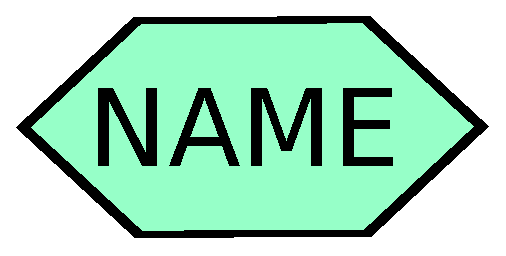
\includegraphics[scale = 0.3]{images/phenotype}
  \caption{The \PD glyph for \glyph{phenotype}.}
  \label{fig:phenotype}
\end{figure}

The example in \fig{phenotype-MPF} illustrates the use of a \glyph{phenotype} node to represent cell division, stimulated by the mono-phosphorylated form of the maturation promoting factor. 

\begin{figure}[H]
  \centering
  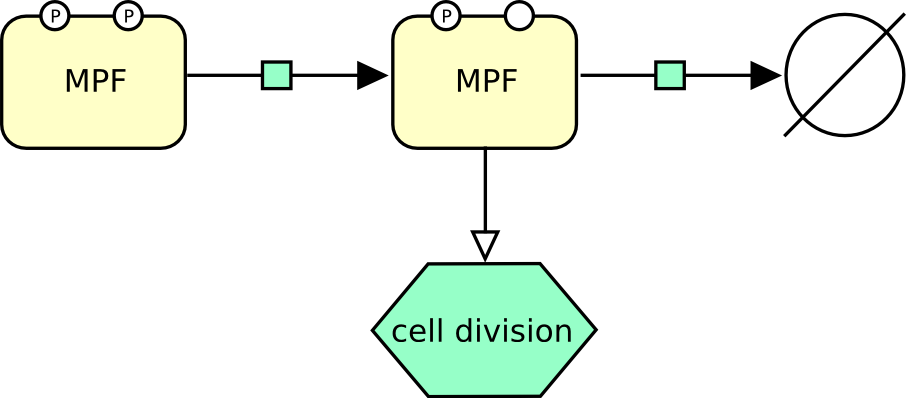
\includegraphics[scale = 0.4]{images/phenotype-MPF}
  \caption{Cell division stimulated by MPF.}
  \label{fig:phenotype-MPF}
\end{figure}
